\section{Experimental evaluation of the Early Stopping algorithm }\label{appendix:evaluation}

To sanity-check the experiments, we present an additional graph of the relationship between NDH and early stopping algorithm reward loss in~\Cref{fig:evaluation-ndh-lostreward}, and the full numerical data for~\Cref{fig:evaluation-envs}. We also show example runs of the experiment in all environments in~\Cref{fig:evaluation-all-one}.

\begin{figure}[htbp]
    \centering
    \begin{subfigure}[b]{0.55\textwidth}
        \centering
        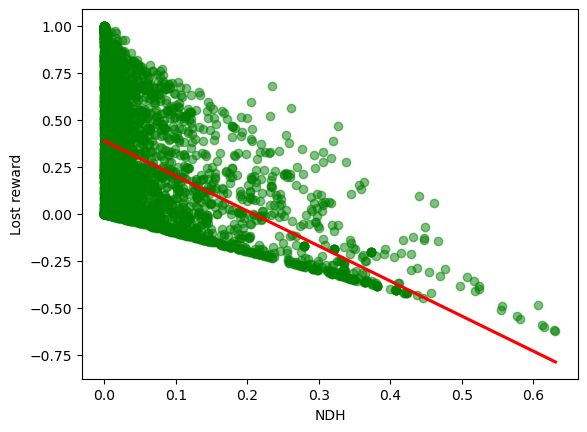
\includegraphics[width=\textwidth]{metrics/lostreward_ndh.png}
    \end{subfigure}
    \caption{The relationship between the amount of Goodharting, measured by NDH, and the amount of reward that is lost due to pessimistic stopping. As Goodharting increases (measured by an increase in NDH), the potential for \emph{gaining} reward by early stopping increases (fitted linear regression shown as the red line. $y = -1.863x  + 0.388$, 95\% CI for slope: $[-1.951, -1.775]$, 95\% CI for intercept: $[0.380, 0.396]$, $R^2 = 0.23$, $p < 1e-10$). Only the points with NDH > 0 are shown in the plot.}
    \label{fig:evaluation-ndh-lostreward}
\end{figure}

\begin{table}[htbp]
\centering
\label{tab:results}
\begin{tabular}{llrrrrrrrr}
\toprule
Environment & &   count &   mean &    std &    min &    25\% &    50\% &    75\% &     max \\
\midrule
Cliff & BR &  2600.0 &  43.82 &  32.89 &  -4.09 &  12.22 &  42.34 &  71.42 &  100.00 \\
        & MCE &  2600.0 &  44.49 &  32.88 & -14.42 &  12.89 &  44.38 &  71.84 &  100.00 \\
Gridworld & BR &  2600.0 &  30.95 &  30.25 & -19.69 &   3.23 &  21.74 &  53.54 &  100.00 \\
        & MCE &  2600.0 &  28.83 &  28.23 & -20.57 &   3.70 &  21.06 &  46.45 &   99.99 \\
Path & BR &  2600.0 &  40.52 &  34.25 & -60.02 &   7.12 &  37.17 &  67.93 &  100.00 \\
        & MCE &  2600.0 &  41.17 &  35.01 & -62.37 &   7.64 &  36.09 &  70.00 &  100.00 \\
RandomMDP & BR &  5320.0 &  10.09 &  19.47 & -42.17 &   0.00 &   0.10 &  14.32 &   99.84 \\
        & MCE &  5320.0 &  10.36 &  19.67 & -42.96 &   0.00 &   0.13 &  14.94 &   99.84 \\
TreeMDP & BR &  1920.0 &  21.16 &  26.83 & -44.59 &   0.11 &   9.14 &  38.92 &  100.00 \\
        & MCE &  1920.0 &  20.11 &  25.95 & -48.52 &   0.08 &   9.56 &  35.61 &  100.00 \\
\bottomrule
\end{tabular}

\caption{A full breakdown of the true reward lost due to early stopping, with respect to the type of environment and training method used. See~\Cref{sec:quantifying_goodharting} for the descriptions of environments and reward sampling methods. 320 missing datapoints are cases where numerical instability in our early stopping algorithm implementation resulted in NaN values.}
\end{table}


\begin{figure}[htbp]
    \centering
    \begin{subfigure}[b]{0.95\textwidth}
        \centering
        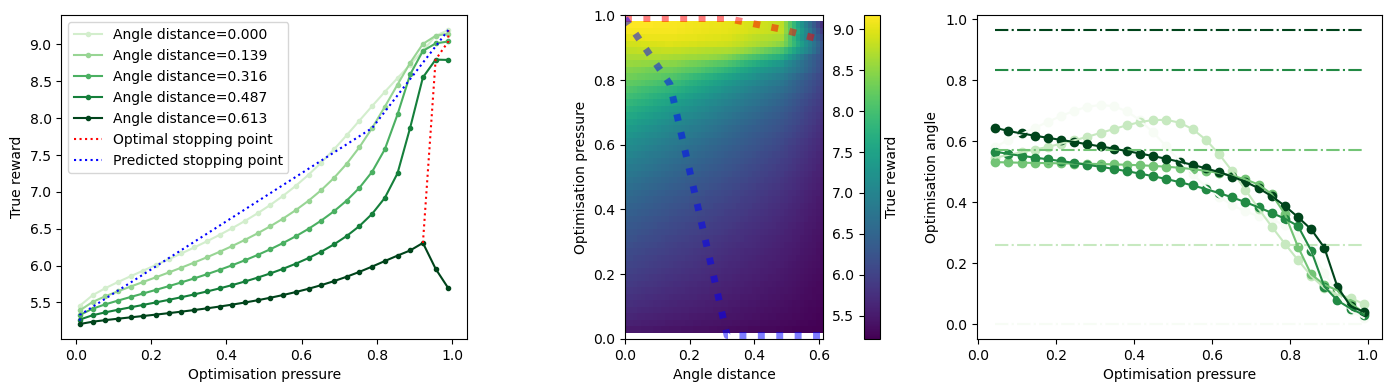
\includegraphics[width=\textwidth]{evaluation/algorithm_example_gridenv.png}
        \caption{\emph{Gridworld} of size 4x4.}
    \end{subfigure}
    \vspace{0.8cm}
    \begin{subfigure}[b]{0.95\textwidth}
        \centering
        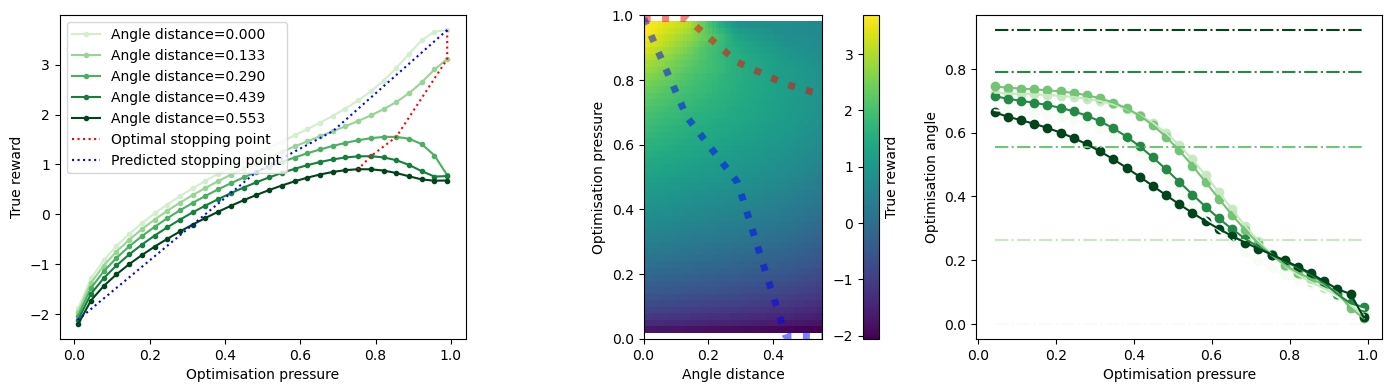
\includegraphics[width=\textwidth]{evaluation/algorithm_example_path.png}
        \caption{\emph{Path} environment of size 4x4.}
    \end{subfigure}
    \vspace{0.8cm}
    \begin{subfigure}[b]{0.95\textwidth}
        \centering
        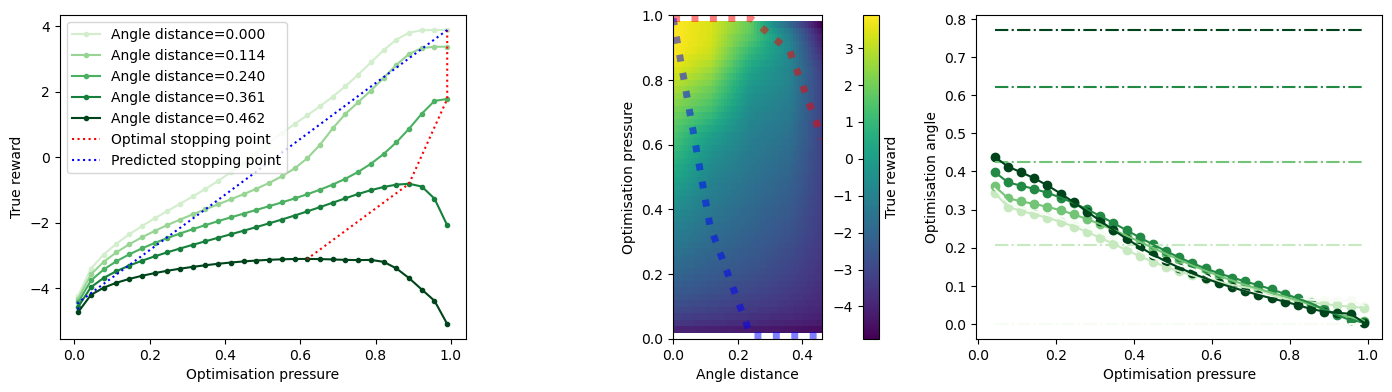
\includegraphics[width=\textwidth]{evaluation/algorithm_example_cliff.png}
        \caption{\emph{Cliff} environment of size 4x4, with a probability of slipping=0.5.}
    \end{subfigure}
    \caption{(Cont. below)}
\end{figure}

\begin{figure}[htbp]\ContinuedFloat
    \centering
    \begin{subfigure}[b]{0.95\textwidth}
        \centering
        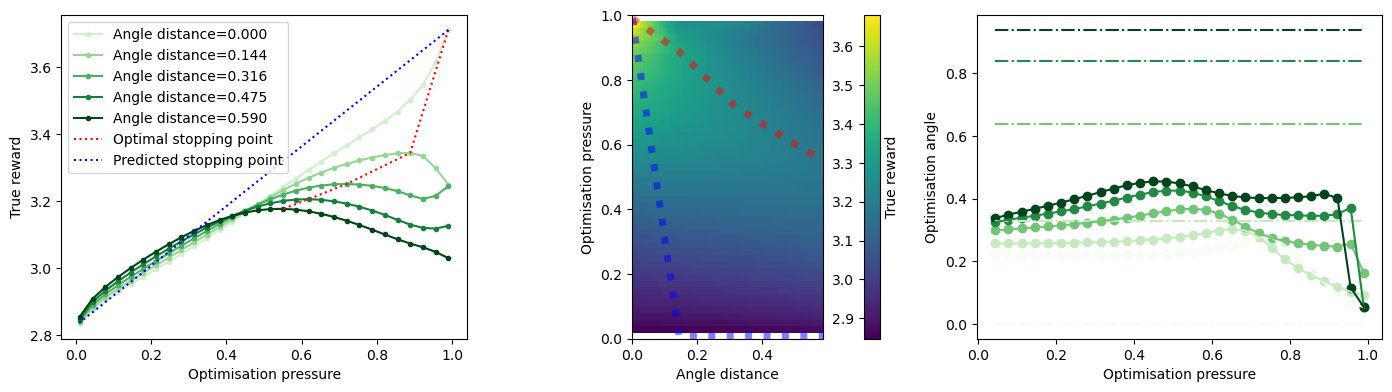
\includegraphics[width=\textwidth]{evaluation/algorithm_example_tree.png}
        \caption{\emph{TreeMDP} of depth=3 and width=2, where terminal states are the 1st and 2nd leaves.}
    \end{subfigure}
    \vspace{0.8cm}
    \begin{subfigure}[b]{0.95\textwidth}
        \centering
        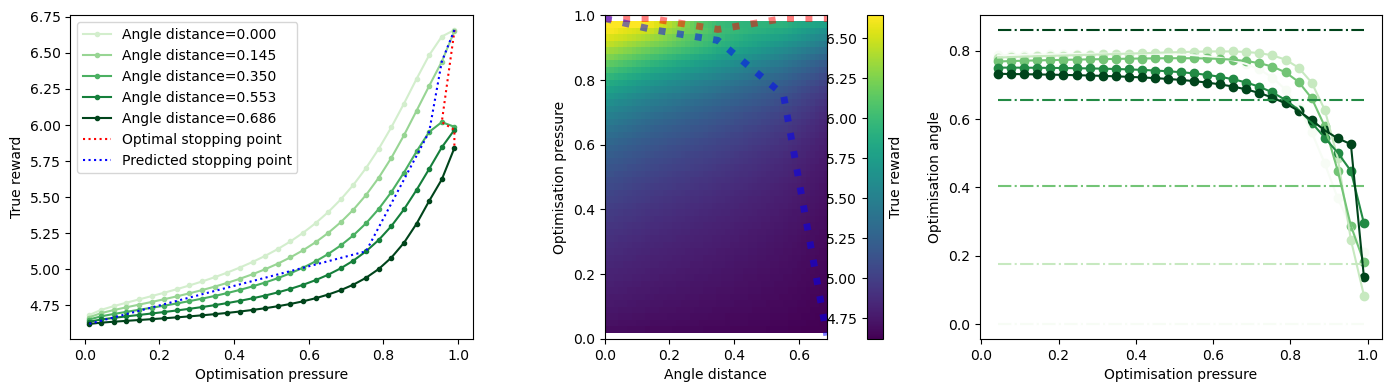
\includegraphics[width=\textwidth]{evaluation/algorithm_example_mdp.png}
        \caption{\emph{RandomMPD} of size=16, with 2 terminal states, and 3 actions.}
    \end{subfigure}
    \vspace{0.8cm}
    \caption{Example runs of the Early Stopping algorithm on different kinds of environments. The left column shows the true reward obtained by training a policy on different proxy rewards, under increasing optimisation pressures.
    The middle column depicts the same plot under a different spatial projection, which makes it easier to see how much the optimal stopping point differs from the pessimistic one recommended by the Early Stopping algorithm.
    The right column shows how the optimisation angle (cosine similarity) changes over increasing optimisation pressure for each proxy reward (for a detailed explanation of this type of plot, see~\Cref{appendix:three-d-example}).\label{fig:evaluation-all-one}}
\end{figure}
